\documentclass[tikz,border=4pt]{standalone}
\usepackage{pgfplots}
\usepackage{times}
\pgfplotsset{compat=1.18}
\begin{document}
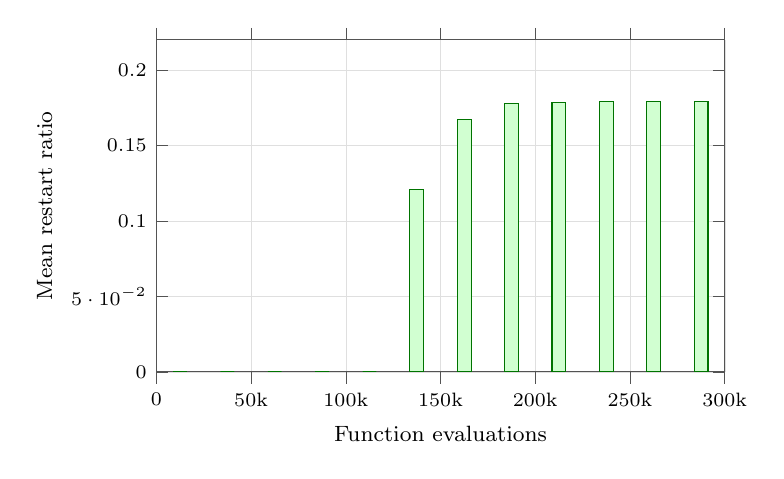
\begin{tikzpicture}
\begin{axis}[
    width=88mm,
    height=58mm,
    xlabel={Function evaluations},
    ylabel={Mean restart ratio},
    xmin=0, xmax=300000,
    ymin=0, ymax=0.22,
    scaled x ticks=false,
    xtick={0,50000,100000,150000,200000,250000,300000},
    xticklabels={0,50k,100k,150k,200k,250k,300k},
    ybar,
    bar width=5pt,
    grid=major,
    grid style={line width=.15pt, draw=gray!25},
    tick label style={font=\scriptsize},
    label style={font=\footnotesize},
    axis line style={gray!65!black},
    tick style={gray!65!black},
]
\addplot+[draw=green!45!black, fill=green!18] coordinates {
(12500,0.0000)
(37500,0.0000)
(62500,0.0000)
(87500,0.0000)
(112500,0.0000)
(137500,0.1211)
(162500,0.1669)
(187500,0.1775)
(212500,0.1784)
(237500,0.1790)
(262500,0.1792)
(287500,0.1792)
};
\end{axis}
\end{tikzpicture}
\end{document}
